% Sample LaTeX document by Adam Přáda
%******************************************************************************
% DOCUMENT AND FONT SET-UP
%******************************************************************************
% First specify the class of document and body font size
\documentclass[11pt]{article}

% Always type input in UTF-8, which guarantees you can write directly most symbols
\usepackage[utf8]{inputenc}

% Next command loads the Latin Modern family of fonts. These look just like LaTeX default Computer Modern, but has more available characters and symbols
\usepackage{lmodern}

% Using the T1 version of the Latin Modern font, better for
\usepackage[T1]{fontenc}

% A generally useful package, e.g. if you want to change font colour
\usepackage{xcolor}

% If writing a document in a different language than English, load the babel package
% Automatically translates words like Chaper, Figure, Table, etc.
%\usepackage[czech]{babel}
%******************************************************************************
% PAGE SET-UP
%******************************************************************************
% Choose the right paper format and margins
%\usepackage[a4paper, top=25mm,bottom=25mm, inner=4cm,outer=3cm]{geometry}
% Each of these can also be set in separate commands
\usepackage{geometry}
\geometry{a4paper}
%\geometry{margin=2.5cm}

% If you want to use multiple columns
%\usepackage{multicol}

% For nicer page headers
%\usepackage{fancyhdr} % Load the package
%\pagestyle{fancy} % Make pages fancy
%\fancyhead[LE,RO]{}
%\fancyhead[RE,LO]{\leftmark}
%\fancyhead[RE,LO]{Section \thesection}
%\fancyfoot[CE,CO]{\leftmark}
%\fancyfoot[LE,RO]{\thepage}
% E: Even page
% O: Odd page
% L: Left field
% C: Center field
% R: Right field
% H: Header
% F: Footer
%******************************************************************************
% PARAGRAPHS
%******************************************************************************
% If you do not want your paragraphs to be indented and you want a gap instead
\setlength{\parindent}{0pt}
\setlength{\parskip}{0.5em}

% If you want to use left or right aligned text, then it may be better to use
% this package,
\usepackage{ragged2e}
% that defines new capitalised commands:
% \Centering
% \RaggedLeft
% \RaggedRight
% These generally work better than their lowercase LaTeX counterparts 
%******************************************************************************
% FIGURES
%******************************************************************************
% For including images/figures
\usepackage{graphicx}
% If most images are in a different folder to the document
\graphicspath{ {figures/} }
%******************************************************************************
% MATHEMATICS
%******************************************************************************
% Basically a necessary package for typing maths
\usepackage{amssymb}
% For more mathematical symbols
\usepackage{amsmath}
% For bold symbols in mathematics
% => use \bm{} instead of \mathbf or \boldsymbol
% => use \hm instead of \heavysymbol
\usepackage{bm}
% Sometimes it may be useful to load the physics package
%\usepackage{physics}
%******************************************************************************
% LINKS IN THE DOCUMENT
%******************************************************************************
% By default I prefer to have links hidden
\usepackage[hidelinks]{hyperref}
% but you can play with them as well
%\usepackage{hyperref}
%\hypersetup{colorlinks=true,linkcolor=black,filecolor=magenta,urlcolor=blue}
%\urlstyle{same}
%******************************************************************************
% BIBTEX BIBLIOGRAPHY
%******************************************************************************
% I prefer to use the Biber backend
%\usepackage[backend=biber,style=chem-rsc,]{biblatex}
%\addbibresource{bibtex/PhD-first-year_report.bib} %Imports bibliography file
%******************************************************************************
% FOOTNOTES WITH SYMBOLS
%******************************************************************************
% I prefer to have footnotes labelled with symbols, to avoid confusion with citations
\renewcommand{\thefootnote}{\fnsymbol{footnote}}
%******************************************************************************
% NON-BREAKING HYPHENS
%******************************************************************************
% Always load as the last package
\usepackage[shortcuts]{extdash}
%Standard LaTeX dashes
%- Standard LaTeX hyphen
%-- Standard LaTeX en-dash
%--- Standard LaTeX em-dash

%extdash breakable dashes
%Words hyphened with these dashes can also be broken at other positions than the dash
%\-/ hyphen
%\-- en-dash
%\--- em-dash

%extdash unbreakable dashes
%No line breaks possible at the hyphen
%\=/ hyphen
%\== en-dash
%\=== em-dash
%******************************************************************************
% DOCUMENT BODY
%******************************************************************************
% If you want to use the default document title, then first set the variables
\title{\LaTeX\ sample}
\author{Adam Přáda}
\date{24 July 2019}
% and then start the document and make the title
\begin{document}
\maketitle
\section{Basics}
Standard text. Standard text. Standard text. Standard text. Standard text. Standard text. Standard text.
Only a full empty line creates a full paragraph break.

paragraph break, paragraph break, paragraph break, paragraph break, paragraph break, paragraph break, paragraph break.

Text can be \textnormal{normal}, a.k.a.~\textrm{roman}, \emph{italics} or \textsl{slanted}, \underline{underlined}, \textsf{without serifs}, \texttt{fixed width}, in \textsc{Small Capitals} or just \uppercase{capitals}, \textbf{bold} or \textmd{medium weight}.

You can also have text of different sizes:

{\Huge Huge}

{\huge huge}

{\LARGE LARGE}

{\Large Large}

{\large large}

{\normalsize normalsize}

{\small small}

{\footnotesize footnotesize}

{\scriptsize scriptsize}

{\tiny tiny}
% These commands act within given scope. In this case it is given by {}
% Can also change and change back or use only within a different object

% You can end the page intentionally like:
\pagebreak
% or
% \newpage
Sometimes you want to use lists:
\begin{itemize}
	\item Item 1
	\item Item 2
	\begin{itemize}
		\item inside item 2
		\item inside item 2
		\begin{itemize}
			\item inside inside
			\item inside inside
		\end{itemize}
		\item inside item 2
	\end{itemize}
	\item Item 3
	\item Item 4
\end{itemize}
or numbered lists
\begin{enumerate}
	\item first
	\item second
\end{enumerate}
\section{Figures}
You also need to have figures, like this nice figure number \ref{fig:qheom_contour}.
\begin{figure} [htp!]
	% h = here
	% t = top of page, can do 'b' for bottom
	% p = separate figure page
	% ! = override default LaTeX settings
	% LaTeX automatically chooses from the options that we list
	\centering
	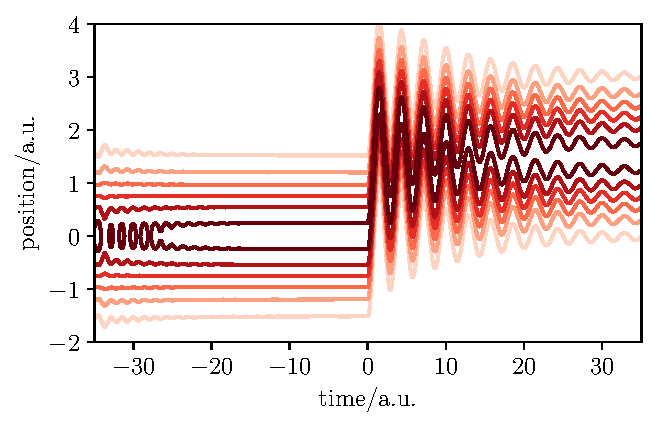
\includegraphics [width=11cm]{qheom_contour.pdf}
	\caption{
		A contour plot of a wavepacket being equilibrated with a bath in a harmonic potential centered at $q=0$. At $t=0$ the potential is shifted by an addition of a linear term, which creates a new minimum at $q=3/2$~a.u. This is a reproduction of a similar calculation from Tanimura, Wolynes, \emph{Phys.~Rev.~A}, 1991, \textbf{43}, 4131–4142.
	}
	\label{fig:qheom_contour}
\end{figure}

\section{Mathematics}
An inline equation $x=3$ inside a paragraph. And a separate equation
\begin{equation}
\hat{\rho}_t(q) = \int \mathrm{d}\bm{x}\langle\bm{x}|\hat{\rho}_t(q,\bm{x}) |\bm{x}\rangle,
\end{equation}
The equation does not have to be numbered like
\begin{equation*}
G_t(q(\tau),q'(\tau)) = \exp\left[\frac{\mathrm{i}}{\hbar}\bigl[S_\mathrm{S}(q(\tau);t)-S_\mathrm{S}(q'(\tau);t)\bigr]\right]
\end{equation*}
but if they are numbered
\begin{equation}
\hat{\rho}_t(q) = \int \mathrm{d}\bm{x}\langle\bm{x}|\hat{\rho}_t(q,\bm{x}) |\bm{x}\rangle,
\label{eq:my_equation}
\end{equation}
then you can refer to them as eq.~\ref{eq:my_equation}. Some equations are long and need two lines
\begin{multline}
\frac{\partial \hat{\rho}_{\bm{n}} }{\partial t} =
-\left(
\frac{\mathrm{i}}{\hbar}\hat{\mathcal{L}}
+\sum_{k=0}^{K}n_k \gamma_k
+\hat{\Xi}
\right)\hat{\rho}_{\bm{n}} \\
-\frac{\mathrm{i}}{\hbar}\hat{q}^\times \sum_{k=0}^{K}\hat{\rho}_{\bm{n}_k^\oplus}
-\frac{\mathrm{i}}{\hbar}\sum_{k=0}^{K}n_k\left(C_k\hat{q}\hat{\rho}_{\bm{n}_k^\ominus}-C_k^*\hat{\rho}_{\bm{n}_k^\ominus}\hat{q}\right),
\end{multline}
Sometimes you want to split the equation, but align it nicely
\begin{equation}
\begin{split}
\frac{\partial \rho_{n}(q_i,q_j) }{\partial t} =
&-\left(\frac{\mathrm{i}}{\hbar}\hat{\mathcal{L}}+n \gamma \right)\rho_{n}(q_i,q_j)
-\frac{\mathrm{i}}{\hbar}(q_i - q_j) \rho_{n+1}(q_i,q_j) \\
&-\frac{n_0 \eta\gamma^2}{2}(q_i + q_j) \rho_{n-1}(q_i,q_j) \\
&-\frac{\mathrm{i}}{\hbar}\frac{n \hbar \eta \gamma^2}{2}\cot\left(\frac{\beta\hbar\gamma}{2}\right)(q_i - q_j) \rho_{n-1}(q_i,q_j).
\end{split}
\end{equation}
Sometimes you want to give people a choice
\begin{equation}
H_\mathrm{S}(q_i,q_j) =
\begin{cases}
V(q_i) +\frac{\hbar^2\pi^2}{6 m (\Delta q)^2}& \text{for }i=j, \\
\frac{\hbar^2 }{m (\Delta q)^2 (i-j)^2}(-1)^{i-j} & \text{otherwise,}
\end{cases}
\label{eq:dvr_ham}
\end{equation}

\end{document}